\documentclass[12pt, a4paper, reqno]{amsart}
\usepackage[slovene]{babel}
\usepackage[T1]{fontenc}
\usepackage[utf8]{inputenc}
\usepackage{amsmath,amssymb,amsfonts,amsthm}
\usepackage{url}
\usepackage[dvipsnames,usenames]{color}
\usepackage{graphicx}
\usepackage{tikz}
\usepackage{dsfont}
\usepackage{caption}
\usepackage{subcaption}
\usepackage{bm}
\usepackage{float}
\usepackage{xcolor}
\usepackage{bbm}
%\usepackage{titlesec}
\allowdisplaybreaks

%--------------------------------------OBLIKA DOKUMENTA--------------------------------------------%

% Oblika strani
\textwidth 15cm
\textheight 24cm
\oddsidemargin.5cm
\evensidemargin.5cm
\topmargin-5mm
\addtolength{\footskip}{10pt}
\pagestyle{plain}
\overfullrule=15pt % oznaci predlogo vrstico

% Naslovi
%\titleformat{\section}
%{\normalfont\Large\bfseries\centering\MakeUppercase}{\thesection}{1em}{}
%
%\titleformat{\subsection}
%{\normalfont\large\bfseries}{\thesubsection}{1em}{}
%
%\titleformat{\subsubsection}
%{\normalfont\normalsize\bfseries}{\thesubsubsection}{1em}{}


% Matematicna okolja (tekst napisan pokoncno)
\theoremstyle{definition}
\newtheorem{definicija}{Definicija}[section]
\newtheorem{zgled}[definicija]{Zgled}
\newtheorem{opomba}[definicija]{Opomba}

\renewcommand\endzgled{\hfill$\diamondsuit$}

% Matematicna okolja (tekst napisan posevno)
\theoremstyle{plain} 
\newtheorem{lema}[definicija]{Lema}
\newtheorem{izrek}[definicija]{Izrek}
\newtheorem{trditev}[definicija]{Trditev}
\newtheorem{posledica}[definicija]{Posledica}



% Ukaz za slovarsko geslo
\newlength{\odstavek}
\setlength{\odstavek}{\parindent}
\newcommand{\geslo}[2]{\noindent\textbf{#1}\hspace*{3mm}\hangindent=\parindent\hangafter=1 #2}

% Podatki o delu
\newcommand{\program}{Finančna matematika} 
\newcommand{\imeavtorja}{Anej Rozman} 
\newcommand{\imementorja}{~doc.~dr. Martin Raič} 
\newcommand{\naslovdela}{Sestavljeni Poissonov proces in njegova uporaba v financah} 
\newcommand{\letnica}{2024} 

% Dodatni ukazi
\newcommand{\R}{\mathbb{R}}
\newcommand{\N}{\mathbb{N}}
\newcommand{\E}{\mathbb{E}}
\newcommand{\F}{\mathcal{F}}
\newcommand{\B}{\mathcal{B}}
\newcommand{\Prob}{\mathbb{P}}
\newcommand{\1}{\mathds{1}}
\newcommand{\Pois}[1]{\text{Pois}(#1)}
\newcommand{\Var}[1]{\text{Var}\left[#1\right]}

%------------------------------------------NASLOVNE STRANI-----------------------------------------%

\begin{document}

\thispagestyle{empty}
\noindent{\large
UNIVERZA V LJUBLJANI\\[1mm]
FAKULTETA ZA MATEMATIKO IN FIZIKO\\[5mm]
\program\ -- 1.~stopnja}
\vfill

\begin{center}{\large
\imeavtorja\\[2mm]
{\bf \naslovdela}\\[10mm]
Delo diplomskega seminarja\\[1cm]
Mentor: \imementorja}
\end{center}
\vfill

\noindent{\large
Ljubljana, \letnica}
\pagebreak

\thispagestyle{empty}
\tableofcontents
\pagebreak

\thispagestyle{empty}
\begin{center}
{\bf \naslovdela}\\[3mm]
{\sc Povzetek}
\end{center}

%--------------------------------------POVZETEK V SLOVENSCINI--------------------------------------%



%--------------------------------------------------------------------------------------------------%

\vfill
\begin{center}
{\bf Compound Poisson process and its application in finance}\\[3mm] 
{\sc Abstract}
\end{center}

%--------------------------------------POVZETEK V ANGLESCINI---------------------------------------%



%--------------------------------------------------------------------------------------------------%

\vfill\noindent
{\bf Math. Subj. Class. (2020):} 60G07 60G20 60G51 \\[1mm]
{\bf Klju"cne besede:} slu"cajni procesi, sestavljeni Poissonov proces,\newline Cramér--Lundbergov model\\[1mm]
{\bf Keywords:} stochastic processes, compound Poisson process, Cramér--Lundberg model
\pagebreak



%--------------------------------------------VSEBINA-----------------------------------------------%

\section{Uvod}

    \begin{center}
        \framebox[\linewidth]{%
    \rule{0pt}{50pt}%
    Uvodni tekst in motivacija za "studiranje procesa, naka"zi da bo"s obravnaval Cramer-Ludenbergov model%
        }
    \end{center}

    \begin{figure}[H]
        \centering
        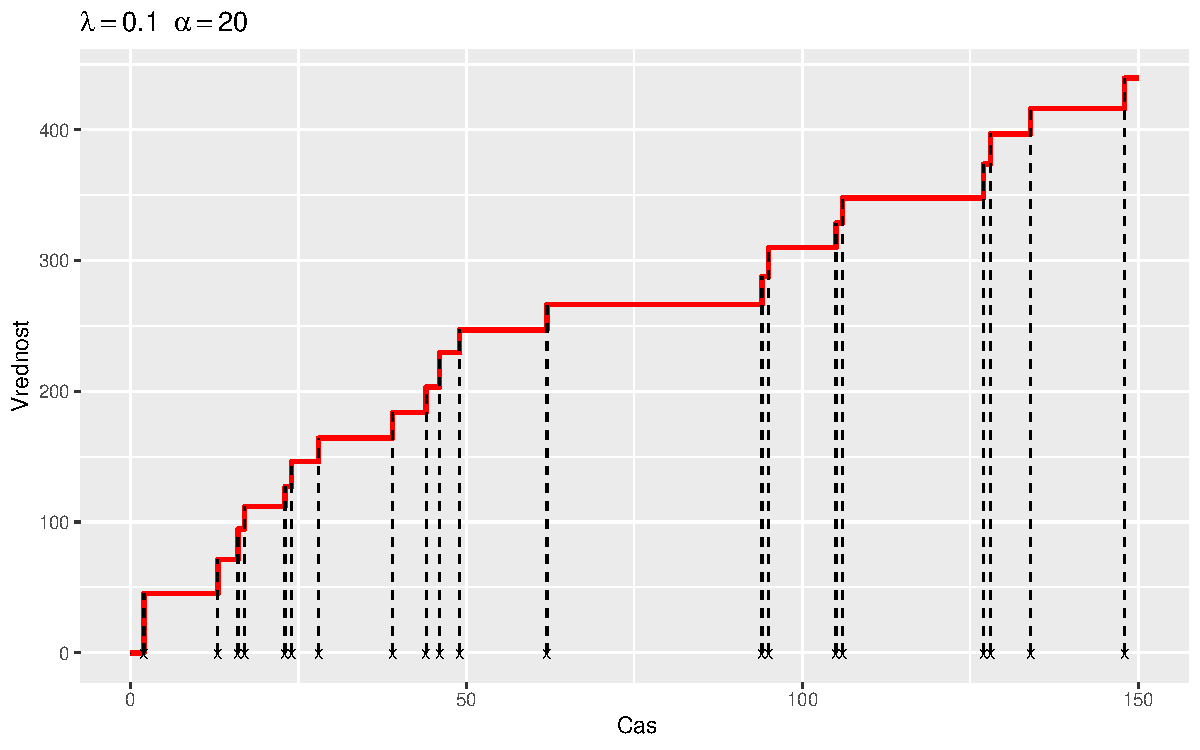
\includegraphics[width=\textwidth]{
            C:/Users/38651/OneDrive - Univerza v Ljubljani/Desktop/Diploma/Diplomski-seminar/GraphsAndPhotos/slika1.pdf
            }
        \caption{Primer trajektorije sestavljenega Poissonovega procesa}
        \label{fig:slika1}
    \end{figure}
    
    \noindent


    \begin{definicija}
        Naj bo $(\Omega, \mathcal{F}, \mathbb{P})$ verjetnostni prostor in naj bo $T\neq\emptyset$
        neprazna indeksna množica ter $(E, \Sigma)$ merljiv prostor. \textit{Slučajni proces}, 
        parametriziran s $T$, je družina slučajnih elementov $X_t : \Omega \to E$,
         ki so $(\mathcal{F}, \Sigma)$-merljivi za vsak $t \in T$.
        \label{def:slucProc}
    \end{definicija}

    \begin{opomba}
        V delu se bomo omejili na primer, ko $T$ predstavlja "cas, torej $T = [0, \infty)$ in da slu"cajne
        spremenljivke 
        zavzemajo vrednosti v realnih "stevilih, torej $(E, \Sigma) = (\R, \B_{\R})$, kjer $\B_\R$ 
        predstavlja Borelovo $\sigma-$algebro na $\R$.
        \label{op:Konvencije}
    \end{opomba}


    \begin{definicija}
        Za fiksen $\omega \in \Omega$ je preslikava 
        $[0, \infty) \rightarrow \mathbb{R}; \ t \mapsto X_t(\omega)$ 
        \textit{trajektorija} oziroma \textit{realizacija} slučajnega procesa $(X_t)_{t\geq0}$.
        Tako lahko slu"cajni proces gledamo kot predpis, ki vsakemu elementu vzor"cnega prostora 
        $\Omega$ priredi slu"cajno funkcijo
        $(X_t(\omega))_{t\geq0}: [0, \infty) \rightarrow \mathbb{R}$.
        \label{def:realizac}
    \end{definicija}

    \begin{definicija}
        Naj bo $(X_t)_{t\geq0}$ slu"cajni proces. Potem za $s < t$ definiramo
        \textit{prirastek procesa} $X_t - X_s$ na intervalu $[s, t]$. Proces $(X_t)_{t\geq0}$ ima 
        \textit{neodvisne prirastke}, če so za vsak nabor realnih "stevil
        $0 \leq t_1 < t_2 < \ldots < t_n < \infty$ prirastki
        $$
            X_{t_2} - X_{t_1}, \ X_{t_3} - X_{t_2}, \ \ldots, \ X_{t_n} - X_{t_{n-1}}
        $$
        med seboj neodvisni.
        \label{def:prirastek}
    \end{definicija}

    \begin{trditev}
        Naj bo $(X_t)_{t\geq0}$ slu"cajni proces na $(\Omega, \F, \mathbb{P})$. Potem ima $(X_t)_{t\geq0}$
        neodvisne prirastke natanko tedaj, ko je za vsak nabor realnih "stevil 
        $0 \leq t_1 < \ldots < t_n < t_{n+1} <\infty$ prirastek $X_{t_{n+1}} - X_{t_n}$ neodvisen od
        slu"cajnega vektorja $(X_{t_1}, \dots, X_{t_n})$.
        \label{trd:ekvivKarakterizacija}
    \end{trditev}

    \begin{proof}
        $(\Rightarrow):$

        $(\Leftarrow):$
    \end{proof}

    \begin{definicija}
        Naj bo $(X_t)_{t\geq0}$ slu"cajni proces. Potem pravimo, da ima proces
        \textit{stacionarne prirastke}, "ce za vsak $s < t$ in vsak $h > 0$ velja, 
        da ima $X_{t+h} - X_{s+h}$ enako porazdelitev kot $X_t - X_s$.
        \label{def:stacPrir}
    \end{definicija}

    \begin{definicija}
        Naj bo $\lambda > 0$. Slučajnemu procesu $(N_t)_{t\geq 0}$, definiranem na verjetnostnem 
        prostoru $(\Omega, \mathcal{F}, \mathbb{P})$ in z vrednostmi v $\N_0$, pravimo 
        \textit{Poissonov proces} z intenzivnostjo $\lambda$, če zadošča naslednjim pogojem:
        \begin{enumerate}
            \item $N_0 = 0$ \ $\Prob$-skoraj gotovo.
            \item $(N_t)_{t\geq 0}$ ima neodvisne in stacionarne prirastke,
            \item Za $0 \leq s < t$ velja $ N_t - N_s \sim\Pois{\lambda(t - s)}$,
        \end{enumerate}
        \label{def:HPP}
    \end{definicija}
\textcolor{red}{
    \begin{opomba}
        Vidimo, da v definiciji ne zahtevamo, da so skoki procesa le +1. To sledi iz...
        \label{op:skoki}
    \end{opomba}
}

\section{Sestavljeni Poissonov proces}

    \begin{center}
        \framebox[\linewidth]{%
    \rule{0pt}{50pt}%
        Povzetek poglavja/krajsi uvod%
        }
    \end{center}
    \begin{definicija}
        Naj bo $(N_t)_{t\geq0}$ Poissonov proces z intenzivnostjo $\lambda$. 
        Naj bo $(X_i)_{i\geq1}$ zaporedje neodvisnih (med sabo in $(N_t)_{t\geq0}$) in enako 
        porazdeljenih slučajnih spremenljivk z vrednostmi v $\mathbb{R}$. Potem je 
        \textit{sestavljeni Poissonov proces} $(S_t)_{t\geq0}$ definiran kot
        $$
            S_t = \sum_{i=1}^{N_t} X_i.
        $$
        \label{def:CPP}
    \end{definicija}

    \begin{opomba}
        Vidimo, da je sestavljeni Poissonov proces posplo"sitev homogenega Poissonovega procesa, saj "ce za
        $X_i$ vzamemo konstantno funkcijo $X_i = 1$ za vsak $i$, dobimo ravno $HPP$. Bolj v splo"snem, "ce za $X_i$ 
        postavimo $X_i = \alpha$, potem velja $S_t = \alpha N_t$.
        \label{op:CPPHPPPovezava}
    \end{opomba}

    V nadaljevanju bomo homogen Poissonov proces z intenzivnostjo $\lambda >0$ ozna"cevali s $HPP(\lambda)$ 
    ali naborom slu"cajnih spremenljivk $(N_t)_{t\geq0}$ (angl. Homogeneous Poisson Process), 
    sestavljeni Poissonov proces pa s $CPP$ ali naborom slu"cajnih spremenljivk $(S_t)_{t\geq0}$ 
    (angl. Compound Poisson Process), kjer bo vsota sledila $HPP(\lambda)$.

    \subsection{Osnovne lastnosti}

        \begin{trditev}
            $CPP$ ima neodvisne in stacionarne prirastke.
            \label{trd:neodvPrirCPP}
        \end{trditev}

        \begin{proof}
            Za nabor realnih "stevil $0 \leq t_1 < t_2 < \ldots < t_n < \infty$ lahko slu"cajne
            spremeljivke $S_{t_i} - S_{t_{i-1}}$ zapi"semo kot
            \begin{align*}
                S_{t_i} - S_{t_{i-1}} &= \sum_{j=N_{t_{i-1}}+1}^{N_{t_i}} X_j. 
            \end{align*}
            Neodvisnost prirastkov sledi po neodvisnosti $X_i$ od $X_j$ za $i\neq j$ in $N_t$. 
            Naj bo $h > 0$ in $s < t$. Potem velja
            \begin{align*}
                S_{t+h} - S_{s+h} &= \sum_{j=N_{s+h}+1}^{N_{t+h}} X_j \\
            \end{align*}
            Vsota ima $N_{t+h} - N_{s+h}$ členov. Ker za $HPP$ velja 
            $N_{t+h} - N_{s+h} \sim N_t - N_s$, je 
            \begin{align*}
                \sum_{j=N_{s+h}+1}^{N_{t+h}} X_j = \sum_{j=N_{s}+1}^{N_{t}} X_j = S_t - S_s.
            \end{align*}
        \end{proof}

        \begin{trditev}
            Naj bo $(S_t)_{t\geq 0}$ $CPP$ in naj bosta $\mu = \E\left[X_i\right] < \infty$ 
            pri"cakovana vrednost in $\sigma^2= \Var{X_i} <\infty$ varianca
            slu"cajnih spremenljivk $X_i$ za vsak $i$. Potem sta za $t\geq0$ pri"cakovana vrednost in 
            varianca $S_t$ enaki 
            \begin{equation*}
                \E\left[S_t\right] = \mu\lambda t \qquad \text{in} \qquad \Var{S_t} = \lambda t\left(\sigma^2 + \mu^2\right).
            \end{equation*}
            \label{trd:PricVarCPP}
        \end{trditev}

        \begin{proof}

            Definiramo slu"cajno spremenljivko
            \begin{equation}
                Y_k = X_1 + X_2 + \cdots + X_k
                \label{eq:Y_k}
            \end{equation}
            in vidimo, da je za $t\geq0$ $S_t$ pogojno na $N_t = k$ enako porazdeljena 
            kot $Y_k$. Tako dobimo 
            \begin{align*}
            \E\left[S_t\mid N_t = k\right] = \E\left[Y_k\right] = k\mu \qquad \text{in} \qquad
            \Var{S_t\mid N_t = k} = \Var{Y_k} = k\sigma^2.
            \end{align*}
            Po formuli za popolno pri"cakovano vrednost velja 
            $\E\left[S_t\right] = \E\left[\E\left[S_t\mid N_t\right]\right]$. Torej

            \begin{align*}
                \E\left[S_t\right] = \E\left[\E\left[S_t\mid N_t\right]\right] = \E\left[\mu N_t\right] = \mu\lambda t.
            \end{align*}

            \noindent
            Prek formule $\Var{S_t} = \E\left[\Var{S_t\mid N_t}\right] + \Var{\E\left[S_t\mid N_t\right]}$ ra"cunamo 

            \begin{equation*}
                \E\left[\Var{S_t\mid N_t}\right] = \E\left[\Var{X_i}N_t\right] = \sigma^2\lambda t
            \end{equation*}
            in 
            \begin{equation*}
                \Var{\E\left[S_t\mid N_t\right]} = \Var{\E\left[X_i\right]N_t} = \mu^2\lambda t,
            \end{equation*}
            saj $N_t\sim\Pois{\lambda t}$. Skupaj dobimo $\Var{S_t} = \lambda t\left(\sigma^2 + \mu^2\right)$.
        \end{proof}

    \subsection{Rodovne funkcije}

    \begin{trditev}
        Naj bo $(S_t)_{t\geq0}$ $CPP$. Naj bodo slu"cajne spremenljivke $X_i$, ki jih se"stevamo v 
        $CPP$ enako porazdeljene kot $X$. Potem ima za $t\geq0$ karakteristi"cna funkcija $\varphi_{S_t}$ 
        obliko
        \begin{equation*}
            \varphi_{S_t}(u) = e^{\lambda t\left(\varphi_X(u) - 1\right)}, 
        \end{equation*}
        kjer $\varphi_X$ ozna"cuje karakteristi"cno funkcijo $X$.
        \label{trd:MomentGener}
    \end{trditev}
    
    \begin{proof}
        \begin{align}
            \varphi_{S_t}(u) 
                    &= \E\left[\exp\left[iuS_t\right]\right] = \nonumber
                        \E\left[\exp\left[iu\sum_{i = 1}^{N_t}X_i\right]\right] \nonumber\\
                    &= \sum_{k=0}^{\infty}
                        \E\left[\exp\left[iu\sum_{i = 1}^{N_t}X_i\mid N_t=k\right]\right]\Prob\left(N_t = k\right) \nonumber \\ 
                    &= \sum_{k=0}^{\infty}
                        \E\left[\exp\left[iu\sum_{i = 1}^kX_i\right]\right]\Prob\left(N_t = k\right) \nonumber \\
                    &= \sum_{k=0}^{\infty}
                        \underbrace{\E\left[e^{iuX}\right]^k}_{\varphi_X(u)^k}\frac{(\lambda t)^k}{k!}e^{-\lambda t} \label{eq:MomentS_t}\\ 
                    &= e^{-\lambda t} + e^{-\lambda t}\sum_{k=1}^\infty\frac{\left(\varphi_X(u)\lambda t\right)^k}{k!} \nonumber \\
                    &= e^{\lambda t\left(\varphi_X(u) - 1\right)} \nonumber
        \end{align}
    \end{proof}

    Hitro lahko vidimo, da sta karakteristi"cna in rodovna funkcija $CPP$ enaki

    \begin{equation*}
        \varphi_{S_t}(u) = e^{\lambda t\left(\varphi_X(u) - 1\right)} \qquad \text{in} \qquad 
        G_{S_t}(u) = e^{\lambda t\left(G_X(u) - 1\right)},
    \end{equation*} 

    \noindent
    saj v splo"snem velja, da je karakteristi"cna funkcija neke slu"cajne spremenljivke $Y$ enaka
    njeni momentno rodovni funkciji izvrednoteni v $iu$, torej $\varphi_Y(u) = G_Y(iu)$. Rodovna pa 
    izverdnotena v $\ln(u)$, torej $G_Y(u) = M_Y(\ln(u))$, "ce obstajata.
    V nadaljevanju bomo uporabljali predvsem karakteristi"cno funkcijo $CPP$, saj je ta vedno definirana 
    za vsak $u\in\R$. Prav nam bo pri"sla tudi naslednja povezava med karakteristi"cno funkcijo $CPP$ 
    in rodovno funkcijo $HPP(\lambda)$.
    \begin{trditev}
        Naj bosta $(S_t)_{t\geq0}$ $CPP$ in $(N_t)_{t\geq0}$ $HPP(\lambda)$ neodvisna. 
        Naj bodo slu"cajne spremenljivke $X_i$, ki jih se"stevamo v $CPP$ enako porazdeljene kot $X$. 
        Potem za fiksen $t\geq0$ velja

        \begin{align*}
            \varphi_{S_t}(u) = G_{N_t}\left(\varphi_{X}(u)\right).
        \end{align*}

        \label{trd:povezavaRodovneKarkateristicne}
    \end{trditev}

    \begin{proof}
        Po ena"cbi (\ref{eq:MomentS_t}) iz trditve \ref{trd:MomentGener} velja, da je $\varphi_{S_t}(u)$ enaka
        \begin{align*}
            \varphi_{S_t}(u) &= \sum_{k=0}^{\infty}
            \varphi_X(u)^n\frac{(\lambda t)^k}{k!}e^{-\lambda t} \\
            &= G_{N_t}\left(\varphi_X(u)\right).
        \end{align*}
    \end{proof}

    \subsection{Porazdelitev CPP}
    Sedaj se posvetimo vpra"sanju, kako je porazdeljena slu"cajna spremenljivka $S_t$ za $t\geq 0$? 
    Iz definicije $HPP(\lambda)$ vemo, da je $N_t$ za $t\geq0$ porazdeljena kot Poissonova slu"cajna 
    spremenljivka s parametrom $\lambda t$. Fiksiramo $t\geq0$ in dobimo 

    \begin{align*}
        F_{S_t}(x) = \Prob(S_t \leq x) 
        &= \sum_{k=0}^\infty \Prob(S_t \leq x \mid N_t = k)\Prob(N_t = k) \\
        & = \sum_{k=0}^\infty \Prob(\sum_{i=1}^k X_i \leq x)\frac{(\lambda t)^k}{k!}e^{-\lambda t} \\
        & = \sum_{k=0}^\infty F_X^{*k}(x)\frac{(\lambda t)^k}{k!}e^{-\lambda t}, \\
    \end{align*}

    \noindent
    kjer je $F_X^{*k}(x)$ porazdelitev $k$-te konvolucije slu"cajne spremenljivke $X$. Razen za 
    posebne primere, je zgornji izraz za prakti"cne namene ne-izra"cunljiv in nam ne pomaga veliko.
    
    \begin{zgled}
        "Ce pogledamo primer, ko so $X_1, X_2, \dots$ neodvisne enako porazdeljene slu"cajne spremenljivke,
        porazdeljene kot $X$
        \begin{equation*}
            X\sim\text{Gamma}(a) \qquad \qquad f_X(x) = \frac{1}{\Gamma(a)}x^{a-1}e^{-x}
        \end{equation*}
        s parametrom $a>0$, lahko pridemo do razmeroma eksplicitne porazdelitve $CPP$. Gostota $k$-te 
        konvolucije $X_1 + \cdots + X_k$ ima formulo
        \begin{equation*}
            f_{X_1 + \cdots + X_k}(x) = \frac{1}{\Gamma(na)}x^{na-1}e^{-x}.
        \end{equation*}
        Za $t\geq 0$ in $x \geq 0$ torej velja
        \begin{align*}
            F_{S_t}(x) = \Prob(S_t \leq x)
            &= \sum_{k=0}^\infty F_X^{*k}(x)\frac{(\lambda t)^k}{k!}e^{-\lambda t}\\
            &= \sum_{k=0}^\infty 
            ...
        \end{align*}

        

    \end{zgled}
    
    %Poka"zimo, da je $CPP$ v resnici porazdeljen, kot limita linearne 
    %kombinacije neodvisnih Poissonovih slu"cajnih spremenljivk. 
    
    \begin{trditev}
        Naj bo $N\sim \Pois{\lambda}$  za $\lambda >0$ in $X_1, X_2, \dots X_n$ neodvisne s.s. (neodvisne 
        med sabo in od $N$) enako porazdeljene kot
        $$ X\sim
        \begin{pmatrix}
            a_1 & a_2 & a_3  \dots & \\
            \tfrac{\lambda_1}{\lambda} & \tfrac{\lambda_2}{\lambda} & \tfrac{\lambda_3}{\lambda} \dots & 
        \end{pmatrix},
        $$
        za poljubne $a_1, a_2, \dots, a_n \in \R$ in 
        $\lambda_1, \lambda_2, \dots, \lambda_n \in \R^+$ za katere velja 
        ${\sum_{i=1}^n\lambda_i = \lambda}$.
        Potem velja 
        \begin{equation*}
            \sum_{j=1}^\infty a_jY_j \sim \sum_{j=1}^NX_j,
        \end{equation*}
        kjer so $Y_1,Y_2,  \dots$ neodvisne s.s.\ porazdeljene kot 
        $\Pois{\lambda_1},\Pois{\lambda_2}, \dots$
        \label{trd:NXjeEnakoaY}
    \end{trditev}

    \begin{proof}
        S $\varphi_{Z_n}(u)$ ozna"cimo karakteristi"cno funkcijo s.s.\ 
        $Z_n := a_1Y_1 + a_2Y_2 + \dots + a_nY_n$ in s $\varphi_{Z}(u)$ karakteristi"cno funkcijo s.s.\
        $Z:= \sum_{j=1}^{N}X_j$. Po neodvisnosti velja
        \begin{align*}
            \varphi_{Z_n}(u) 
                    &= \prod_{j=1}^{n}\varphi_{Y_j}(a_ju)\\
                    &= \prod_{j=1}^{n}\exp\left[\lambda_j\left(e^{a_j i u} - 1\right)\right] \\
                    &= \exp\left[\sum_{j=1}^{n}\lambda_j\left(e^{a_j i u} - 1\right)\right].
        \end{align*}

        \noindent
        Po trditvi \ref{trd:povezavaRodovneKarkateristicne} velja
        \begin{align*}
            \varphi_{Z}(u) 
                    &= G_N\left(\varphi_X(u)\right) \\
                    &= \exp\left[\lambda\left(\varphi_X(u) - 1\right)\right] \\
                    & = \exp\left[\lambda\left(\sum_{j=1}^\infty\frac{\lambda_j}{\lambda}e^{a_jiu} - 1\right)\right]\\
                    &= \exp\left[\sum_{j=1}^{\infty}\lambda_j\left(e^{a_j i u} - 1\right)\right]
        \end{align*}

        \noindent 
        Vidimo, da velja%Rezultat je posledica inverzne formule za karateristi"cne funkcije.
        \begin{equation*}
            \varphi_{Z_n} \xrightarrow{n\to\infty}\varphi_Z,
        \end{equation*}
        torej po Lévijevem izreku o kontinuiteti velja $Z_\infty :=\lim_{n\to\infty}Z_n \sim Z$.
    \end{proof}

    \begin{posledica}
        Naj bo $(a_n)_{n\in\N}$ poljubno zaporedje realnih "stevil in $(\lambda_n)_{n\in\N}$ zaporedje 
        pozitivnih realnih "stevil, za katere velja $\sum_{n=1}^\infty\lambda_n = \lambda$ in 
        \begin{equation*}
            X\sim
            \begin{pmatrix}
                a_1 & a_2 &  \dots \\
                \tfrac{\lambda_1}{\lambda} & \tfrac{\lambda_2}{\lambda} & \dots
            \end{pmatrix}.
        \end{equation*}
        Potem velja
        \begin{equation*}
            \sum_{j=1}^{n}a_jY_j \xrightarrow[n\to\infty]{d}\sum_{j=1}^NX_j,
        \end{equation*}
        \label{pos:NXjeEnakoaYstevno}
    \end{posledica}

    \begin{proof}
        Ker velja $\varphi_{Z_n}(u) \xrightarrow{n\to\infty} \varphi_{Z}(u)$ za vsak $u\in\R$, po Lévijevem
        izreku o zveznosti sledi, da $Z_n \xrightarrow[n\to\infty]{d} Z$.
    \end{proof}

    Kaj pa v primeru, ko so $X_i$ zvezno porazdeljene? 
    Tedaj se problema lotimo na slede"c na"cin. Definiramo $F_n(x) := F(\tfrac{m}{n})$ kjer je
    $F(x)$ porazdelitvena funkcija slu"cajne spremenljivke $Z_n$ in 
    $m = \min\{k \in \mathbb{Z} \mid \tfrac{k}{n} > F_n(x)\}$.

        \begin{figure}[H]
            \begin{center}
            
                \begin{tikzpicture}
                    % coordinate system
                    \draw[->] (-0.75,0) -- (9,0) node[right] {$x$};
                    \draw[->] (2,0) -- (2,4.5) node[above] {$F, F_n$};
                    \draw (2, 3.4) -- (2, 3.4) node[left] {$1$};
                    \draw[dashed] (-0.75,3.2) -- (9,3.2);
                
                    % CDF of continuous random variable
                    \draw[blue] (-0.75, 0.1) .. controls (0,0.2) and (2.2, 0.3) .. (2.8, 1.2);
                    \draw[->, blue] (2.8, 1.2) .. controls (3.1, 1.7) and (3.6, 2) .. (5, 2.1);
                    \filldraw[blue] (5, 2.5) circle (0.7pt);
                    \draw[blue] (5, 2.5) .. controls (6, 2.8) and (7.5, 3) .. (9, 3.15) node[below] {$F(x)$};
                
                    % CDF of F_n, 
                    \draw[->, red] (-0.75, 0.22) -- (0.25, 0.22);
                    \filldraw[red] (-0.75, 0.22) circle (0.7pt);
                    \draw[->, red] (0.25, 0.39) -- (1.25, 0.39);
                    \filldraw[red] (0.25, 0.39) circle (0.7pt);
                    \draw[->, red] (1.25, 0.74) -- (2.25, 0.74);
                    \filldraw[red] (1.25, 0.74) circle (0.7pt);
                    \draw[->, red] (2.25, 1.68) -- (3.25, 1.68);
                    \filldraw[red] (2.25, 1.68) circle (0.7pt);
                    \draw[->, red] (3.25, 2.01) -- (4.25, 2.01) node[above left]{$F_n(x)$};
                    \filldraw[red] (3.25, 2.01) circle (0.7pt);
                    \draw[->, red] (4.25, 2.58) -- (5.25, 2.58);
                    \filldraw[red] (4.25, 2.58) circle (0.7pt);
                    \draw[->, red] (5.25, 2.79) -- (6.25, 2.79);
                    \filldraw[red] (5.25, 2.79) circle (0.7pt);
                    \draw[->, red] (6.25, 2.94) -- (7.25, 2.94);
                    \filldraw[red] (6.25, 2.94) circle (0.7pt);
                    \draw[->, red] (7.25, 3.07) -- (8.25, 3.07);
                    \filldraw[red] (7.25, 3.07) circle (0.7pt);
                
                
                    %intervals of F_n
                
                \end{tikzpicture}
                \caption{Aproksimacija $F$ s $F_n$}
                \label{fig:slika2}
            \end{center}
        \end{figure}

    \noindent
    Kot je razvidno iz slike \ref{fig:slika2}, je $F_n(x)$ stopni"casta funkcija, ki aproksimira 
    porazdelitveno funkcijo $F(x)$. Velja $F_n \xrightarrow{n\to\infty}F$ povsod kjer je $F$ zvezna.



    %\noindent
    %"Ce sedaj po"sljemo $n \to \infty$, dobimo
    %\begin{align}
    %    \varphi_{Z}(u) := \lim_{n\to\infty}\varphi_{Z_n}(u) = e^{\sum_{j=1}^{\infty}\lambda_j\left(e^{a_j i u} - 1\right)}.
    %    \label{eq:karFunkcVrste}
    %\end{align}
%
    %\noindent
    %Kot smo izpeljali zgoraj je karakteristi"cna funkcija $CPP$ podana s predpisom
%
    %\begin{align*}
    %    \varphi_{S_t}(u) = e^{\lambda t\left(\varphi_X(u) - 1\right)}, 
    %\end{align*}
%
    %\noindent
    %kar lahko zapi"semo kot 
%
    %\begin{align*}
    %    \varphi_{S_t}(u) = e^{\lambda t\int_{\R}\left(e^{i u z} - 1\right) \mu(dz)},
    %\end{align*}
%
    %\noindent
    %kjer je $\mu := X*\Prob$ potisk mere naprej po s.s.\ $X$. Prav tako lahko (\ref{eq:karFunkcVrste}) zapi"semo
    %kot 
%
    %\begin{align*}
    %    \varphi_{Z}(u) = e^{\int_{\R}\left(e^{i u x} - 1\right)\nu(dx)},
    %\end{align*}
%
    %\noindent
    %Za neko ustrezno mero $\nu$. Vidimo, da ko po"sljemo $n\to \infty$, za ustrezen izbor 
    %$a_1, a_2, \dots$ in $\lambda_1, \lambda_2, \dots$ karakteristi"cna funkcija 
    %vrste $Z_n$ konvergira h karakteristi"cni funkciji $S_t$. Torej po Lévijevem izreku o zveznosti 
    %sledi, da je $S_t$ enako porazdeljena kot $Z = \sum_{i=1}^{\infty}\alpha_iY_i$.
%

    \subsection{CPP kot martingal}

        \begin{definicija}
            Slu"cajni proces $X_t$ prilagojen glede na filtracijo $(\F_t)_{t\geq0}$
            martingal, "ce velja 
            $$
                \E\left[X_t\mid\F_s\right] = X_s
            $$
            za vsak $0\leq s \leq t$.
            \label{def:martingal}
        \end{definicija}

        Poka"zimo, da v splo"snem $CPP$ ni martingal.

        \begin{trditev}
            Naj bo $(S_t)_{t\geq0}$ $CPP$ z intenzivnostjo $\lambda>0$ in naj bodo $X_i$ neodvisne
            in enako porazdeljene slu"cajne spremenljivke z $\E\left[X_i\right] = \mu$ za vsak $i$.
            Potem je $S_t$ martingal natanko tedaj, ko je $\mu = 0$.
            \label{trd:CPPnimartingal}
        \end{trditev}

        \begin{proof}
            Naj bo $0\leq s\leq t$. Potem velja
            \begin{align*}
                \E\left[S_t\mid\F_s\right] 
                        &= \E\left[S_t - S_s + S_s\mid \F_s\right] \\
                        &= \E\left[S_t - S_s\right] + \E\left[S_s\mid \F_s\right] \\
                        &= \mu\lambda(t-s) + S_s
            \end{align*}
           Enakost $\mu\lambda(t-s) + S_s = S_s$ velja $\iff$ $\mu\lambda(t-s) = 0 \iff \mu = 0$.
        \end{proof}

        \begin{opomba}
            Seveda, "ce velja $\mu \geq 0$, potem je $S_t$ submartingal, "ce pa $\mu \leq 0$, je
            $S_t$ supermartingal.
        \end{opomba}

        \begin{trditev}
            Naj bo $(S_t)_{t\geq0}$ CPP z intenzivnostjo $\lambda > 0$ in naj bodo $X_i$ neodvisne
            in enako porazdeljene slu"cajne spremenljivke z $\E\left[X_i\right] = \mu$ za vsak $i$,
            Potem je proces 
            $$
                S_t - \mu\lambda t
            $$
            martingal.
            \label{trd:CPPpostanemartingal}
        \end{trditev}

        \begin{proof}
            Naj bosta $0 \leq s < t$. Prirastek $S_t - S_s$ je neodvisen od $\F_s$ in ima 
            pri"cakovano vrednost $\mu\lambda(t-s)$. Torej 
            \begin{align*}
                \E\left[S_t - \mu\lambda t\mid\F_s\right] 
                        &= \E\left[S_t - S_s\right] + S_s - \mu\lambda t\\
                        &= \mu\lambda(t-s) + S_s - \mu\lambda t\\
                        &= S_s - \mu\lambda s.
            \end{align*}
        \end{proof}

        %\subsection{"Cas prvega prehoda}
        %Postavimo si vpra"sanje, kdaj bo $CPP$ prvi"c dosegel nek $a\in\R$. Obravnavajmo primer, ko je 
        %$a>0$, saj je primer, ko je $a$ negativen simetri"cen. Naj bo $T_a = \inf\{t\geq0; S_t \geq a\}$ 
        %"cas prvega prehoda $CPP$. V tem poglavju bomo izra"cunali porazdelitev $T_a$.
        %"Ce pogledamo dogodek $\{T_a \leq t\}$.

\section{Cramér-Lundbergov model}

    V tem razdelku obravnavamo najbolj intenzivno raziskan model v teoriji propada, običajno imenovan 
    Cramér-Lundbergov model. V svoji najosnovnejši obliki 
    ga je v zgodnjih 1900. letih izpeljal "svedski aktuar Filip Lundberg, da bi ocenil ranljivost 
    zavarovalnice za propad. Čeprav je model v svoji ideji dokaj preprost, 
    lepo zajema bistvo dinamike ravni rezerv zavarovalne družbe in njene izpostavljenosti tveganju, 
    kar pojasnjuje, zakaj je postal temeljni merilni model v teoriji propada.
    V preteklem stoletju je bilo razvitih veliko tehnik za analizo Cramér-Lundbergovega modela, 
    ki so se večinoma osredotočile na kvantifikacijo verjetnosti propada. V razdelku podamo 
    pregled glavnih rezultatov in osnovnih tehnik, ter jih ponazorimo na primerih, ko 
    zavarovalni"ske zahtevke modeliramo z lahkorepimi in te"zkorepimi porazdelitvami.

    \subsection{Proces tveganja in verjetnost propada}

        \begin{definicija}
            Naj bo $(S_t)_{t\geq0 }$ $CPP$.\ \textit{Proces tveganja} v Cramér-Lundbergovem modelu definiramo kot
            \begin{align*}
                U_t = u + p(t) - S_t,
            \end{align*}
            kjer je $u \geq 0$ za"cetni kapital zavarovalnice in $p(t)$ funkcija prihodkov iz premij. 
            \label{def:procesTveganja}
        \end{definicija}

        \begin{opomba}
            V resnici lahko veliko lastnosti procesa tveganja izpeljemo brez da predpostavimo, da prihodi 
            zahtevkov v $(S_t)_{t\geq0}$ sledijo Poissonovemu procesu,
            ampak splo"snemu prenovitvenemu procesu (\ref{def:PrenovitveniProces}) in
            zato na za"cetku ne bomo uporabljali rezultatov, ki smo jih do sedaj izpeljali.
            \label{op:procesTveganja}
        \end{opomba}

        Vrednost $U_t$ predstavlja kapital zavarovalnice ob "casu $t\geq0$. Standardno je za $p(t)$ 
        vzeti deterministi"cno funkcijo $p(t) = ct$, kjer je $c>0$ stopnja prihodkov premij.
        Uporaba linearne funkcije za modeliranje premijskega dohodka v Cramér-Lundbergovem 
        modelu ponuja realističen približek zato, ker zavarovalnice pogosto doživljajo 
        stabilno povečevanje premijskega dohodka skozi čas. Poleg tega je izbira linearne 
        funkcije preprosta, zato bomo v nadaljevanju privzeli, da je $p(t) = ct$. Poglejmo si 
        realizaciji procesa tveganja, ko so zahtevki $X_i$ porazdeljeni Weibullovo 
        (\ref{def:WeibullovaPorazdelitev}) z razli"cnimi parametri. 

        \begin{zgled}
            Naj bo $(U_t)_{t\geq0}$ proces tveganja v Cramér-Lundbergovem modelu z za"cetnim kapitalom
            $u = 1000$ in $p(t) = 200t$ ter intenzivnostjo prihodov zahtevkov $\lambda=1$. % v $CPP$. 
            Naj bodo v prvem primeru (rde"ca) 
            zahtevki porazdeljeni kot $X_i \sim \text{Weibull}(2, 434)$ in v drugem primeru (modra) kot
            $Y_i \sim \text{Weibull}(\tfrac{1}{4}, 16)$.
            
            \begin{figure}[H]
                \centering
                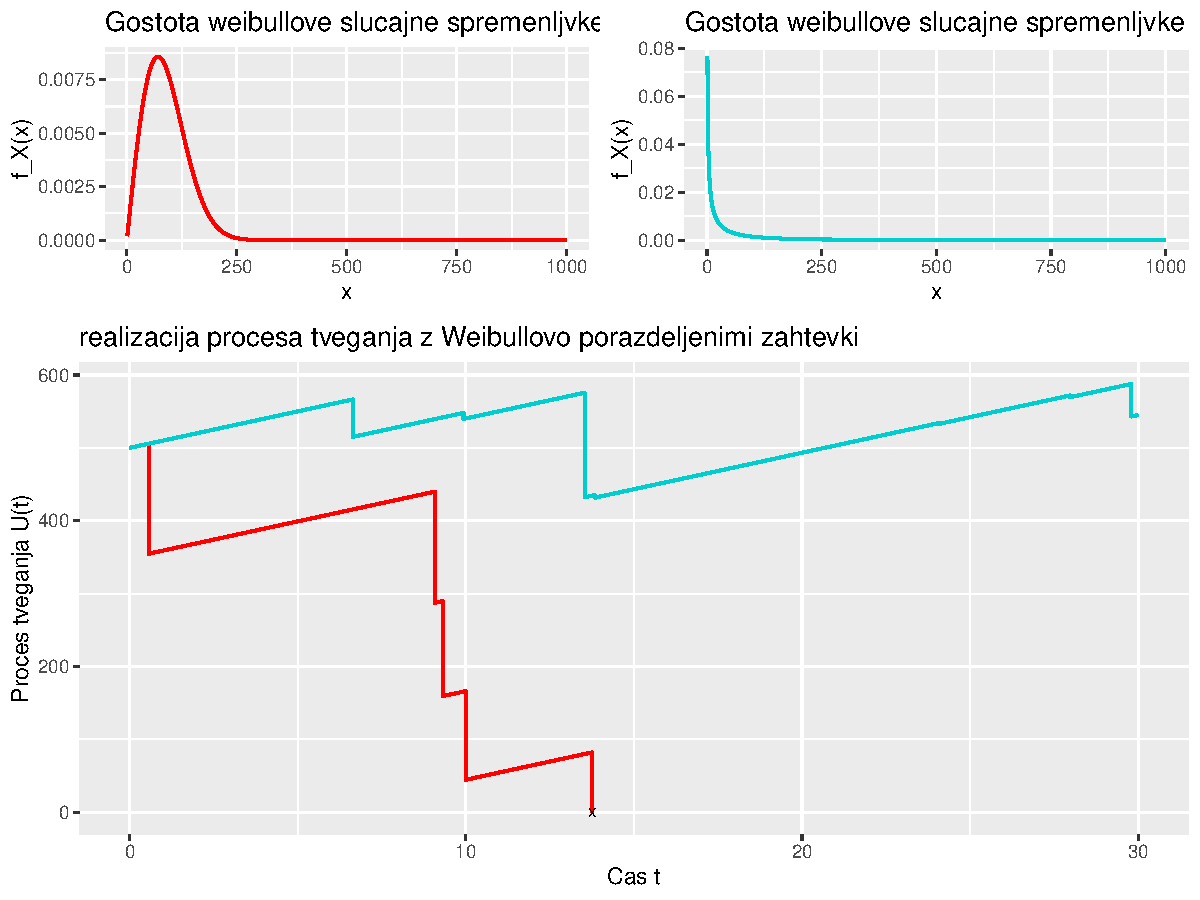
\includegraphics[width=\textwidth]{
                    C:/Users/38651/OneDrive - Univerza v Ljubljani/Desktop/Diploma/Diplomski-seminar/GraphsAndPhotos/slika2.pdf
                    }
                \caption{Realizaciji procesa tveganja}
                \label{fig:slika3}
            \end{figure}

            Pri obeh realizacijah vidimo, da proces tveganja v nekem trenutku pade pod $0$ (tam ga 
            tudi ustavimo). "Ceprav je pri"cakova vrednost 
            $\E\left[Y_i\right] = 384 \approx \E\left[X_i\right] = 217\sqrt{\pi} \approx 384,62$ 
            opazimo bistveno razliko med realizacijama. V rde"cem primeru proces pade pod
            $0$ po ve"c zaporednih manj"sih izgubah, v modrem primeru pa po eni zelo veliki izgubi. 
            V nadaljevanju bomo primera lo"cili, ampak pred tem 
            definirajmo kako obravnavamo dogodek, ko proces tveganja pade pod $0$.

            \label{zgd:weibullProcesTveganja}
        \end{zgled}

        \begin{definicija}
            \textit{Propad} definiramo kot dogodek, da proces tveganja $(U_t)_{t\geq0}$ kadarkoli pade pod $0$. 
            Torej 
            \begin{align*}
                \bigl\{U_t<0 \ \text{za} \ t\geq 0\bigr\}
            \end{align*}
            in "casu
            \begin{align*}
                T = \inf\{t\geq0 \mid U_t < 0\}, 
            \end{align*}
            pravimo \textit{"cas propada}. Seveda velja enakost med dogodkoma
            \begin{align*}
                \{U_t<0 \ \text{za} \ t\geq0\} = \{T<\infty\}.
            \end{align*}
            \label{def:PropadCasPropada} 
        \end{definicija}

        \begin{definicija}
            \textit{Verjetnost propada} je definirana kot funckija $\psi(u): (0,\infty) \to [0,1]$ 
            podana s predpisom
            \begin{align*}
                \psi(u) = \Prob(T<\infty \mid U_0 = u).
            \end{align*}
            \label{def:VerjetnostPropada}
        \end{definicija}

        \begin{definicija}
            Po konstrukciji procesa tveganja $(U_t)_{t\geq0}$ je verjentost propada mogo"ca le ob 
            prihodih zahtevkov. %, ki sledijo $HPP(\lambda)$
            S $T_n$ ozna"cimo "cas $n$-tega prihoda in definiramo 
            \textit{ogrodje procesa tveganja} kot $(U_{T_n})_{n\in\N}$.
            \label{def:ogrodjeProcesaTveganja}
        \end{definicija}

        \begin{trditev}
            Naj bo $(U_t)_{t\geq0}$ proces tveganja v Cramér-Lundbergovem modelu in $(U_{T_n})_{n\in\N}$ 
            njegovo ogrodje ter $W_n := T_n - T_{n-1}$ medpirhodni "cas $n$-tega zahtevka 
            $(W_0 = T_0 = 0)$. Potem velja 
            \begin{equation*}
                \psi(u) = \Prob\left(\sup_{n\in\N}Z_n > u\right),
            \end{equation*}
            kjer je $Z_n = \sum_{i=1}^nY_i$  komulativna izguba po $n$ prihodih in $Y_i = X_i - cW_i$
            izguba $i$-tega prihoda.
            \label{trd:verjetnostPropadaZOgrodjem}
        \end{trditev}

        \begin{proof}

            S pomo"cjo ogrodja procesa tveganja lahko dogodek propada zapi"semo kot
            \begin{align*}
                \biggl\{\inf_{t\geq0}U_t<0\biggr\} &= \biggl\{\inf_{n\in\N}U_{T_n}<0\biggr\} \\
                              &= \biggl\{\inf_{n\in\N}\bigl\{u + p(T_n) - S_{T_n}\bigr\} < 0\biggr\} \\
                              &= \biggl\{\inf_{n\in\N}\biggl\{u + 
                              \underbrace{cT_n - \sum_{i=1}^nX_i}_{-Z_n}\biggr\} < 0\biggr\} \\
                              &= \biggl\{\inf_{n\in\N}\{-Z_n\} < -u\biggr\} \\
                              &= \biggl\{\sup_{n\in\N}Z_n > u\biggr\},
            \end{align*}
            kar nam da "zeljeno enakost.
        \end{proof}

        Tako verjetnost propada prevedemo na prehodno verjetnost diskretnega slu"cajnega 
        sprehoda $(Z_n)_{n\in\N}$. V nadaljevanju nas bo predvsem zanimalo asimptoti"cno 
        vedenje $\psi(u)$, ko gre $u\rightarrow\infty$. Cilj obravnavanja verjetnosti propada v 
        Cramér-Lundbergovem modelu je, da se izognemo 
        propadu z verjetnostjo 1 oziroma, da je verjetnost, da $(Z_n)_{n\in\N}$ prese"ze $u$
        tako majhna, da lahko v praksi dogodek propada izklju"cimo. 


        \begin{trditev}
            Naj bo $(Z_n)_{n\in\N}$ zaporedje slu"cajnih spremenljivk definirano kot 
            $Z_n = \sum_{i=1}^nY_i$ za neodvisne in enako porazdeljene slu"cajne spremenljivke 
            $Y_i$ z $\E\left[Y_i\right] = \mu < \infty$. Potem za vsak $u>0$ velja
            \begin{equation*}
                \Prob\left(\sup_{n\in\N}Z_n > u\right) = 1 \quad \text{za} \ u > 0,
            \end{equation*}
            "ce velja $\E\left[Y_i\right] \geq 0$.
            \label{trd:propadZVerjetnostjo1}
        \end{trditev}

        \begin{proof}
            Zaporedje slu"cajnih spremenljivk $(Y_i)_{i\in\N}$ zadostuje krepkemu zakonu velikih 
            "stevil (\ref{izr:KrepkiZakonVelikihStevil}), torej velja
            \begin{equation*}
                \frac{Y_1 + Y_2 + \cdots Y_n}{n} = \frac{Z_n}{n} \xrightarrow[n\to\infty]{s.g.} \E\left[Y_n\right].
            \end{equation*}
            Torej bo $Z_n$ v primeru ko je $\mu>0$
             skoraj gotovo asimptoti"cno linearno nara"scal proti $\infty$ kot $\mu n$ in 
             bo za poljuben $u>0$
            \begin{equation*}
                \Prob\left(\sup_{n\in\N}Z_n > u\right) = 1.
            \end{equation*}
            Dokaz za primer, ko je $\mu = 0$ je precej bolj tehni"cen in ne preve"c informativen, zato 
            ga bomo izpustili. Lahko ga najdemo v [Spitzer, 138].
        \end{proof}

        \begin{opomba}
            Iz trditve \ref{trd:propadZVerjetnostjo1} (ob predpostavkah $\E\left[X_i\right] < \infty$
            in $\E\left[W_i\right] < \infty$) sledi, da moramo premijo $c$ izbrati tako, da bo 
            $\E\left[Y_i\right] < 0$, saj je to edini na"cin, ko lahko upamo, da verjetnost propada ne bo
            enaka 1.
            \label{op:izbiraPremije}
        \end{opomba}
    
        %V nadaljevanju bomo
        %predpostavili, da sta $\E\left[X_n\right]$ in $\E\left[W_n\right]$ kon"cni. To nam 
        %zagotovi, da je $\E\left[Z_n\right] = \sum_{i=1}^n\E\left[X_i\right] - c\E\left[W_i\right]$
        %kon"cna.
%
        %Ker pa velja ena od treh mo"znosti:
        %\begin{align*}
        %    \E\left[Y_n\right] = 
        %    \begin{cases}
        %        > 0, & \text{za} \ c\E\left[W_n\right] > \E\left[X_n\right], \\
        %        = 0, & \text{za} \ c\E\left[W_n\right] = \E\left[X_n\right], \\
        %        < 0, & \text{za} \ c\E\left[W_n\right] < \E\left[X_n\right],
        %    \end{cases}
        %\end{align*}
%
        %\noindent
        %bo verjetnost propada enaka 1, "ce velja $\E\left[Y_n\right] > 0$, saj $(Z_n)_{n\in\N}$ 
        %zadostuje predpostavkam krepkega zakona velikih "stevil.
        %\begin{equation*}
        %    \frac{Z_n}{n} \xrightarrow[n\to\infty]{s.g.} \E\left[Y_n\right] > 0.
        %\end{equation*}
        %Vidimo torej, da bo $Z_n$ skoraj gotovo linearno nara"scal proti $\infty$ in bo za poljuben 
        %$u>0$
        %\begin{equation*}
        %    \Prob\left(\sup_{n\in\N}Z_n > u\right) = 1.
        %\end{equation*}
%
        %Izka"ze se da celo v 
        %primeru ko bo $\E\left[Y_n\right] = 0$ bo verjetnost propada enaka 1, ker bosta obstajali 
        %pozdaporedji $(n_k)_{k\in\N}$ in $(m_k)_{k\in\N}$... Spitzer [138] je dokazano.

        \begin{definicija}
            Pravimo, da proces tveganja $(U_t)_{t\geq0}$ v Cramér-Lundbergovem modelu
             zadostuje \textit{pogoju neto zaslu"zka} (ang. \textit{net profit condition}), "ce velja 
            \begin{equation*}
                c > \frac{\E\left[X\right]}{\E\left[W\right]} \quad \text{oziroma} \quad 
                c = (1 + \rho)\frac{\E\left[X\right]}{\E\left[W\right]} \quad \text{za $\rho > 0$}.
            \end{equation*}
            Pogoj bomo v nadaljenvanju imenovali NPC.
            \label{def:NPC}
        \end{definicija}

        Zahteva NPC za analizo poslovanja zavarovalnice je kar intuitivna, saj pove, da mora v 
        neki "cavni enoti biti pri"cakoan dohodek iz premij ve"cji od pri"cakovanega izpla"cila zahtevkov.

        \begin{zgled}[Nadaljevnaje zgleda \ref{zgd:weibullProcesTveganja}]
            V zgledu \ref{zgd:weibullProcesTveganja} smo obravnavali proces tveganja v Cramér-Lundbergovem 
            modelu, kjer so zahtevki (rde"ca) $X_i\sim\text{Weibull}(2, 434)$ in (modra) 
            $Y_i\sim\text{Weibull}(\tfrac{1}{4}, 16)$. Opazili smo, da je v prvem primeru propad
            posledica ve"c manj"sih izgub, v drugem pa ene velike izgube. Razlog za to je ta, da
            ima Weibullova porazdelitev za $a \geq 1$ lahkorepno, za $a<1$ pa te"zkorepno porazdelitev.
            \begin{proof}
                Momentno rodovna funkcija $X\sim\text{Weibull}(a, b)$ je enaka
                \begin{align*}
                    M_X(u) &= \int_{0}^{\infty}e^{ux}\frac{a}{b}\left(\frac{x}{b}\right)^{a-1}e^{-\left(\frac{x}{b}\right)^a}dx \qquad \left(y = \tfrac{x}{b},\ dy = \tfrac{dx}{b}\right) \\
                           &= \int_{0}^{\infty}e^{uby}a y^{a-1}e^{-y^a}dy.
                \end{align*}
                Vidimo, da je zgornji integral kon"cen za $a\geq 1$ in divergira za $a<1$, "ce v 
                nadaljevanju predpostavimo $a\geq 1$ in uvedemo $z = y^a$, $dz = ay^{a-1}dy$ dobimo \phantom{\qedhere}
                \begin{align*}
                    M_X(u) &= \int_{0}^{\infty}e^{ubz^{\frac{1}{a}}}e^{-z}dz \\
                           &= \int_{0}^{\infty}\sum_{k=0}^{\infty}\frac{(ubz^{\frac{1}{a}})^k}{k!}e^{-z}dz \qquad \qquad \text{Tonelli} \ \ref{izr:TonellijevIzrek} \\
                           &= \sum_{k=0}^{\infty}\frac{(ub)^k}{k!}\int_{0}^{\infty}z^{\frac{k}{a}}e^{-z}dz \\
                           &= \sum_{k=0}^{\infty}\frac{(ub)^k}{k!}\Gamma\left(\frac{k}{a} + 1\right).
                \end{align*} 
            \end{proof}
            \label{zgd:weibullLahkorepnaPorazdelitev}
        \end{zgled}
    
    \subsection{Lahkorepe porazdelitve}
        \subsubsection{Lundbergova neenakost}
            Od sedaj naprej bomo predpostavili, da je $S_t$ v procesu tveganja $(U_t)_{t\geq0}$ $CPP$.
            Najprej se bomo omejili na primer, ko ima porazdelitev slu"cajnih spremenljivk $X_i$, ki jih 
            se"stevamo v $CPP$ lahek rep, saj je bila osnovna teorija, ki sta jo razvila Cramér in Lundberg,
            izpeljana pod to predpostavko.

            \begin{definicija}
                Pravimo, da ima slu"cajna spremenljivka $X$ \textit{lahkorepno porazdelitev}, "ce velja
            \begin{equation*}
                \E\left[e^{uX}\right] = M_X(u) < \infty \quad \text{za} \ u \in (-\varepsilon, \varepsilon)
            \end{equation*}
            za nek $\varepsilon > 0$. Sicer pravimo, da ima $X$ \textit{te"zkorepno porazdelitev}.
            \label{def:lahkorepnaPorazdelitev}
            \end{definicija}

            \begin{opomba}
                V praksi z lahkorepnimi porazdelitvami modeliramo zahtevke, kjer verjentosti ekstremnih 
                dogodkov (torej zelo velikih zahtevkov) eksponentno pada proti $0$. To direktno sledi iz 
                definicije \ref{def:lahkorepnaPorazdelitev} in neenakosti Markova \ref{trd:neenakostMarkova}, 
                saj za vsak 
                $x>0$ in $u\in(-\varepsilon, \varepsilon)$ velja
                \begin{equation*}
                    \Prob\left(X > x\right) = \Prob\left(e^{uX} > e^{ux}\right) \leq \frac{\E\left[e^{uX}\right]}{e^{ux}}.
                \end{equation*}
                \label{op:lahkorepnaPorazdelitev}
            \end{opomba}

            \begin{definicija}
                Naj velja, da ima slu"cajna spremenljivka $Y_1$ iz trditve \ref{trd:verjetnostPropadaZOgrodjem} 
                lahek rep. "Ce obstaja pozitivna
                enoli"cna re"sitev ena"cbe
                \begin{equation*}
                    M_{1Y_1}(\ell)  = 1,
                \end{equation*}
                "stevilu $\ell$ pravimo \textit{Lundbergov koeficient}.
            \end{definicija}

            \begin{trditev}
                mogo"ce dokazi da je $\ell$ res enoli"cna re"sitev.
            \end{trditev}

            \begin{izrek}(Lundbergova neenakost)
                Naj bo $(U_t)_{t\geq0}$ proces tveganja v Cramér-Lundbergovem modelu, ki zadostuje NPC in 
                naj zanj obstaja Lundebrgov koeficient $\ell$. Potem za vsak $u>0$ velja
                \begin{equation*}
                    \psi(u) \leq e^{-\ell u}.
                \end{equation*}
                \label{izr:LundbergovaNeenakost}
            \end{izrek}

            \begin{proof}
                Neenakost bomo dokazali z indukcijo. Za $u>0$ in $n\in\N$ definiramo
                \begin{equation*}
                    \psi_n(u) = \Prob\left(\max_{1\leq k\leq n}Z_k > u\right)
                \end{equation*}
                in vidimo, da je (po zveznosti $\mathbb{P}$ od spodaj) $\psi(u) = \lim_{n\to\infty}\psi_n(u)$, 
                torej moramo pokazati, da za vsak $n\in\N$ velja $\psi_n(u) \leq e^{-\ell u}$. \\
                (n = 1): Kot v opombi \ref{op:lahkorepnaPorazdelitev} uporabimo neenakost Markova in dobimo
                \begin{equation*}
                    \psi_1(u) = \Prob\left(e^{\ell Z_1} > e^{\ell u}\right) \leq \frac{M_{Z_1}(\ell)}{e^{\ell u}} = e^{-\ell u}.
                \end{equation*}
                (n $\rightarrow$ n+1): 
                Ozna"cimo s $F_{Y_1}$ porazdeliltev $Y_1$. Potem velja
                \begin{align*}
                    \psi_{n+1}(u) &= \Prob\left(\max_{1\leq k\leq n+1}Z_k > u\right) \\
                                  &= \underbrace{\Prob\left(Y_1 > u\right)}_{(i)} + 
                                  \underbrace{\Prob\left(\max_{2\leq k\leq n+1}\bigl\{Y_1 + (Z_k - Y_1)\bigr\} > u, Y_1 \leq u\right)}_{(ii)} \\
                \end{align*}
                Najprej se posvetimo $(ii)$. Po indukcijski predpostavki velja 
                \begin{align*}
                    (ii) &= \int_{(-\infty, u]}\Prob\left(\max_{1\leq k\leq n}\bigl\{x + Z_k\bigr\} > u\right)dF_{Y_1}(x) \\
                         &= \int_{(-\infty, u]}\Prob\left(\max_{1\leq k\leq n}Z_k > u - x\right)dF_{Y_1}(x) \\
                         &\stackrel{\text{\scalebox{0.8}{I.P.}}}{=} \int_{(-\infty, u]}\psi_n(u - x)dF_{Y_1}(x) \\
                         &\leq \int_{(-\infty, u]}e^{-\ell(u - x)}dF_{Y_1}(x). \\
                \end{align*}
                Za oceno $(i)$ kot v primeru $n=1$ uporabimo neenakost Markova in dobimo
                \begin{equation*}
                    (i) = \psi_1(u) = \int_{(u, \infty)}dF_{Y_1}(x) \leq \int_{(u, \infty)}e^{\ell (x - u)}dF_{Y_1}(x).
                \end{equation*}

                "Ce torej se"stejemo $(i)$ in $(ii)$ dobimo "zeljeno oceno
                \begin{align*}
                    \psi_{n+1}(u) &\leq \int_{\R}e^{\ell (x - u)}dF_{Y_1}(x) \\
                                  &= e^{-\ell u}M_{Y_1}(\ell) \\
                                  &= e^{-\ell u}.
                \end{align*}

            \end{proof}

            \begin{opomba}
                Iz izreka \ref{izr:LundbergovaNeenakost} je razvidno, da z dovolj visokim za"cetnim kapitalom
                $u$ verjetnost propada lahko v praksi zadovoljivo omejimo blizu $0$. Seveda je meja 
                odvisna tudi od Lundbergovega koeficienta $\ell$ in krepko temelji na predpostavki 
                lahkorepnih porazdelitev, ki pa v praksi pogosto niso izpolnjene.
                \label{op:LundbergovaNeenakost}
            \end{opomba}

            \begin{zgled}
                Naj bo $(U_t)_{t\geq0}$ proces tveganja v Cramér-Lundbergovem modelu, ki zadostuje NPC.\ Naj 
                nadalje velja da so $X_i$ eksponentno porazdeljene slu"cajne spremenljivke s parametrom $\mu$ 
                $(X_i \sim \text{Exp}(\mu) \ \text{za vsak} \ i)$. Vemo, da ima momentno rodovna funkcija 
                $X_i$ obliko 
                \begin{equation}
                    M_{X_i}(u) = \frac{\mu}{\mu - u} \ \text{za} \ u<\mu.
                    \label{eq:MRExsponentneSS}
                \end{equation}
                Tako dobimo, da ima momentno rodovna funkcija $Y_1 = X_1 - cW_1$ obliko 
                \begin{equation*}
                    M_{Y_1}(u) = M_{X_1}(u)M_{W_1}(-cu) = 
                    \frac{\mu}{\mu - u}\frac{\lambda}{\lambda + cu} \ \text{za} \ u\in (-\tfrac{\lambda}{c}, \mu).
                \end{equation*}
                Sedaj lahko izra"cunamo Lundbergov koeficient $\ell$
                \begin{align*}
                    M_{Y_1}(\ell) &= 1, \\
                    \frac{\mu}{\mu - \ell}\frac{\lambda}{\lambda + c\ell} &= 1, \\
                    \mu\lambda &= (\mu - \ell)(\lambda + c\ell), \\
                    \mu\lambda &= \mu\lambda - \ell\lambda + \mu c - c\ell^2, \\
                    0 &= \mu c - c\ell - \lambda.
                \end{align*}
                Dobimo 
                \begin{equation*}
                    \ell = \mu - \frac{\lambda}{c} \in (0, \mu),
                \end{equation*}
                saj v na"sem modelu velja NPC pogoj
                \begin{equation*}
                    \frac{\E\left[X_1\right]}{\E\left[W_1\right]} = \frac{\lambda}{\mu} < c \iff \mu > \frac{\lambda}{c}.
                \end{equation*}
                "Ce uporabimo alternativno formulacijo NPC pogoja, dobimo
                \begin{align*}
                    c = (1 + \rho)\frac{\lambda}{\mu} \Rightarrow
                    \ell = \mu - \frac{\lambda}{(1 + \rho)\frac{\lambda}{\mu}} = \mu\left(\frac{\rho}{1 + \rho}\right).
                \end{align*}
                Tako dobimo zgornjo mejo za verjetnost propada
                \begin{equation*}
                    \psi(u) \leq e^{-\ell u} = e^{-\mu u\left(\frac{\rho}{1 + \rho}\right)}
                \end{equation*}
                in vidimo, da pove"canje premije "cez neko mejo ne bistveno vpliva na oceno, saj 
                \begin{equation*}
                    \lim_{\rho\to\infty}e^{-\mu u\left(\frac{\rho}{1 + \rho}\right)} = e^{-\mu u}.
                \end{equation*}
                V nadaljevanju bomo videli, da je Lundbergova neenakost v primeru eksponentno 
                porazdeljenih zahtevkov skoraj to"cna vrednost verjetnosti propada, zgre"sena le za konstanto.
                V splo"snem pa je zelo te"zko dolo"citi Lunbergov koeficient kot funkcijo parametrov
                porazdelittev $X_1$ in $W_1$ in zato uporabljamo numeri"cne metode za njegovo aproksimacijo 
                kot na primer Monte Carlo simulacije. 
                \label{zgd:LundebrgovaNeenakostEksponentno}
            \end{zgled}

        \subsubsection{Cramérjeva meja za propad}
            Sedaj se bomo posvetili enemu najpomembnej"sih rezultatov v teoriji propada.

            \begin{definicija}
                Za la"zjo notacijo v nadaljevanju definiramo funkcijo \textit{verjentosti pre"zivetja} kot
                $\theta(u):(0, \infty) \to [0, 1]$ s predpisom
                \begin{equation*}
                    \theta(u) = \Prob\left(T=\infty\mid U_0=u\right) = 1 - \psi(u).
                \end{equation*}
                \label{def:verjetnostPrezivetja}
            \end{definicija}

            \begin{lema}
                Naj bo $(U_t)_{t\geq0}$ proces tveganja v Cramér-Lundbergovem modelu, ki zadostuje NPC in naj 
                velja $\E\left[X\right]<\infty$ ter, da je $F_X$ absolutno zvezna glede na Lebesgueovo mero $\mathcal{L}$.
                Potem $\theta(u)$ zado"sca naslednji enakosti
                \begin{equation}
                    \theta(u) = \theta(0) + \frac{1}{(1+\rho)\E\left[X\right]} \int_{(0, u]}\biggl((1 - F_X(x))\theta(u - x)\biggr)dx.
                    \label{eq:verjetnostPrezivetja}
                \end{equation}
                \label{lema:verjetnostPrezivetja}
            \end{lema}

            \begin{proof}
                Po trditvi \ref{trd:verjetnostPropadaZOgrodjem} velja
                \begin{equation*}
                    \psi(u) = \Prob\left(\sup_{n\in\N}Z_n > u\right),
                \end{equation*}
                kjer je $Z_n = \sum_{i=1}^nY_i$ in $Y_i = X_i - cW_i$. Torej je
                \begin{align*}
                    \theta(u) &= \Prob\left(\sup_{n\in\N}Z_n \leq u\right) \\
                              &= \Prob\left(\{Z_n \leq u\mid \forall n\in\N\}\right) \\
                              &= \Prob\left(\{Y_1 \leq u\}\cap \{Z_n - Y_1 \leq u - Y_1\mid \forall n\geq2\}\right) \\
                              &= \E\left[\mathbbm{1}_{\{Y_1\leq u\}}\Prob\left(\{Z_n - Y_1 \leq u - Y_1\mid \forall n\geq2\}\mid Y_1\right)\right].
                \end{align*}
                Sedaj upo"stevamo, da je $Y_1 = X_1 - cW_1$ in je torej dogodek $\{Y_1 \leq u\}$ 
                enak dogodku $\{X_1 \leq u + cW_1\}$. Poleg tega velja, da je 
                $(Z_n - Y_1)_{n\geq2} \sim (Z_n)_{n\in\N}$, saj so $Y_i$ neodvisne in enako porazdeljene.
                Upo"stevamo "se, da je tokrat $W_1$ medprihodni "cas v $HPP(\lambda)$ in je torej 
                eksponentno porazdeljen.
                Tako dobimo

                \begin{align*}
                        \theta(u)   &= \int_{(0, \infty)}\int_{(0, u + cw]}\Prob\left(\{Z_n \leq u - (x - cw)\mid \forall n\in\N\}\right)dF_{X_1}(x)\lambda e^{-\lambda w}dw. \\
                                    &= \int_{(0, \infty)}\int_{(0, u + cw]}\theta(u - x + cw)dF_{X_1}(x)\lambda e^{-\lambda w}dw.
                \end{align*}
                Uvedemo novo spremenljivko $z = u + cw$ (torej $w = \tfrac{z - u}{c}$ in $dw = \tfrac{dz}{c}$) 
                ter dobimo

                \begin{align*}
                            \theta(u) = \frac{\lambda}{c}e^{\tfrac{\lambda u}{c}}\int_{(u, \infty)}e^{\tfrac{-\lambda z}{c}}\underbrace{\int_{(0, z)}\theta(z - x)dF_{X_1}(x)}_{g(z)}dz.
                \end{align*}
                Ker ima porazdelitev $F_X$ gostoto je funkcija $g(z)$ zvezna in celo odvedljiva, ker...
                $\theta(u)$ lahko tako odvajamo in dobimo

                \begin{equation*}
                    \theta'(u) = \frac{\lambda}{c}\theta(u) - \frac{\lambda}{c}\int_{(0, u)}\theta(u - x)dF_{X_1}(x).
                \end{equation*}
                "Ce sedaj obe strani integriramo po $u$ dobimo
                
                \begin{equation}
                    \int_{(0, t]}\theta'(u)du = \frac{\lambda}{c}\int_{(0, t]}\theta(u)du - \frac{\lambda}{c}\int_{(0, t]}\underbrace{\int_{(0, u)}\theta(u - x)dF_{X_1}(x)}_{(i)}du, 
                    \label{eq:verjetnostPrezivetjaIntegral}
                \end{equation}
                Na integralu $(i)$ uporabimo per partes ($\alpha = \theta(u-x)$ in $d\beta = dF_{X_1}(x)$) in dobimo

                \begin{align*}
                    (i)     &= \left(\theta(u - x)F_X(u)\right)\Big|_{0}^{u} + \int_{(0, u)}\theta'(u - x)F_X(x)dx \\
                            &= \theta(0)F_X(u) - \int_{(0, u)}\theta'(u - x)F_X(x)dx.
                \end{align*}
                Kjer upo"stevamo da je $F_X(0) = 0$ saj je $X > 0$ skoraj gotovo. Vstavimo $(i)$ v
                ena"cbo (\ref{eq:verjetnostPrezivetjaIntegral}) in dobimo

                \begin{equation*}
                    \theta(t) - \theta(0) = \frac{\lambda}{c}\int(0, t]\theta(u)du - \frac{\lambda}{c}\int_{(0, t]}\theta(0)F_X(u)du - \frac{\lambda}{c}\int_{(0, t]}\int_{(0, u)}\theta'(u - x)F_X(x)dxdu. 
                \end{equation*}
                Po Tonellijevem izreku \ref{izr:TonellijevIzrek} lahko zamenjamo vrstni red integracije in dobimo

                \begin{align*}
                    \theta(t) - \theta(0) &= \frac{\lambda}{c}\int_{(0, t]}\theta(u)du - \frac{\lambda}{c}\int_{(0, t]}\theta(0)F_X(u)du - \frac{\lambda}{c}\int_{(0, t]}\int_{(x, t)}\theta'(u - x)F_X(x)dudx, \\
                    \theta(t) - \theta(0) &= \frac{\lambda}{c}\int_{(0, t]}\theta(u)du - \frac{\lambda}{c}\int_{(0, t]}\theta(0)F_X(u)du - \frac{\lambda}{c}\int_{(0, t]}F_X(x)(\theta(t-x) - \theta(0))dx,\\
                    \theta(t) &= \theta(0) + \frac{\lambda}{c}\int_{(0, t]}\theta(u)du - \frac{\lambda}{c}\int_{(0, t]}\theta(0)F_X(u)du - \frac{\lambda}{c}\int_{(0, t]}F_X(x)\theta(t-x)dx.
                \end{align*}
                "Ce sedaj upo"stevamo enakost 
                \begin{equation*}
                    \frac{\lambda}{c} = \frac{1}{1 + \rho}\frac{1}{\E\left[X\right]}
                \end{equation*}
                in spremenimo oznake $t\to u$ in $x\to y$ dobimo "zeljeno enakost 
                (\ref{eq:verjetnostPrezivetja}).







            \end{proof}

            \begin{opomba}
                    Ena"cbo (\ref{eq:verjetnostPrezivetja}) lahko zapi"semo tudi v obliki 
                    \begin{equation*}
                        \theta(u) = \theta(0) + \frac{1}{(1+\rho)}\int_{(0, u]}\theta(u - x)dF_X^I(x)
                    \end{equation*}
                    kjer je $F_X^I(x)$ podana z ena"cbo 
                    \begin{equation*}
                        F_X^I(x) = \frac{1}{\E\left[X\right]}\int_{(0, x]}(1 - F_X(y))dy. \ \text{za} \ x>0.
                    \end{equation*}
                    Hitro lahko preverimo, da je $F_X^I(x)$ porazdelitvena funkcija, saj je $F_X^I(0) = 0$, 
                    $F_X^I(x)$ je nara"s"cajo"ca in $F_X^I(x) \uparrow 1$ za $x\to\infty$, ker velja 
                    $\E\left[X\right] = \int_{(0, \infty)}(1 - F_X(x))dx.$ Po osnovnem izreku analize pa 
                    neposredno sledi enakost.
                \label{op:verjetnostPrezivetja}
            \end{opomba}

            \begin{izrek}(Cramérjeva meja za propad)
                Naj bo $(U_t)_{t\geq0}$ proces tveganja v Cramér-Lundbergovem modelu, ki zadostuje NPC in 
                naj zanj obstaja Lundbergov koeficient $\ell$. Naj bo $F_{X}$ porazdelitev slu"cajnih spremenjlvk
                $X_i$, ki je absolutno zvezna glede na Lebesgueovo mero $\mathcal{L}$.\ Potem obstaja konstanta $C>0$ da
                velja 
                \begin{equation*}
                    \lim_{u\to\infty}e^{\ell u}\psi(u) = C.
                \end{equation*}
                \label{izr:CramerjevaMeja}
            \end{izrek}

            \begin{proof}
                TRIVIALNO
            \end{proof}

            \begin{zgled}[Nadaljevnaje zgleda \ref{zgd:LundebrgovaNeenakostEksponentno}]
                Vemo, da re"sitve prenovitvene ena"cbe iz izreka \ref{izr:CramerjevaMeja} v splo"snem ne moremo izra"cuanti.
                V zgledu \ref{zgd:LundebrgovaNeenakostEksponentno} smo pa privzeli, da zahtevke modeliramo 
                z eksponentno porazdelitvijo, torej $X_i\sim\text{Exp}(\mu)$. 
                V tem primeru se izka"ze, da lahko explicitno izra"cunamo verjentost propada 
                \begin{equation}
                    \psi(u) =  \frac{e^{-u\mu\left(\frac{\rho}{1 + \rho}\right)}}{1 + \rho},
                \label{eq:eksplicitnaVerjetnostPropadaExp}
                \end{equation}
                ampak to je zelo poseben primer, ko lahko vse izra"cunamo eksplicitno.\ 
                Poka"zimo, kako bi do pribli"zka lahko prisli z Monte Carlo simulacijami.

                Recimo, da v na"sem modelu pridemo do sklepa, da zahtevki prihajajo z intenzivnostjo
                $\lambda = 1$ in so eksponentno porazdeljeni s parametrom $\mu = 1$, ter da prejemamo 
                premije s konstantno stopnjo $c = 1$. Vemo, 

            \end{zgled}
        
    \subsection{Te"zkorepe porazdelitve}
        \begin{izrek}
            Naj bo $(U_t)_{t\geq0}$ proces tveganja v Cramér-Lundbergovem modelu, ki zadostuje NPC in naj 
            velja $\E\left[X\right]<\infty$ ter, da je $F_X$ absolutno zvezna glede na Lebesgueovo mero $\mathcal{L}$. Naj velja "se, da je porazdelitev $F_X^I$ te"zkorepna. Potem velja 
            \begin{equation}
                \lim_{u\to\infty}\frac{\psi(u)}{1 - F_X^I(u)} = \frac{1}{\rho}.
                \label{eq:tezkorepnePorazdelitveAsimptotika}
            \end{equation}
            \label{izr:tezkorepnePorazdelitveAsimptotika}
        \end{izrek}

        \begin{proof}
            TRIVIALNO
        \end{proof}



        
    %\subsection{Modeliranje realnih podatkov}
    %
    %    V tem razdelku bomo analizirali podatke iz zavarovalni"stva in jih primerjali z rezultati, 
    %    ki smo jih izpeljali v prej"snjih razdelkih. 
%
    %    \begin{figure}[H]
    %        \centering
    %        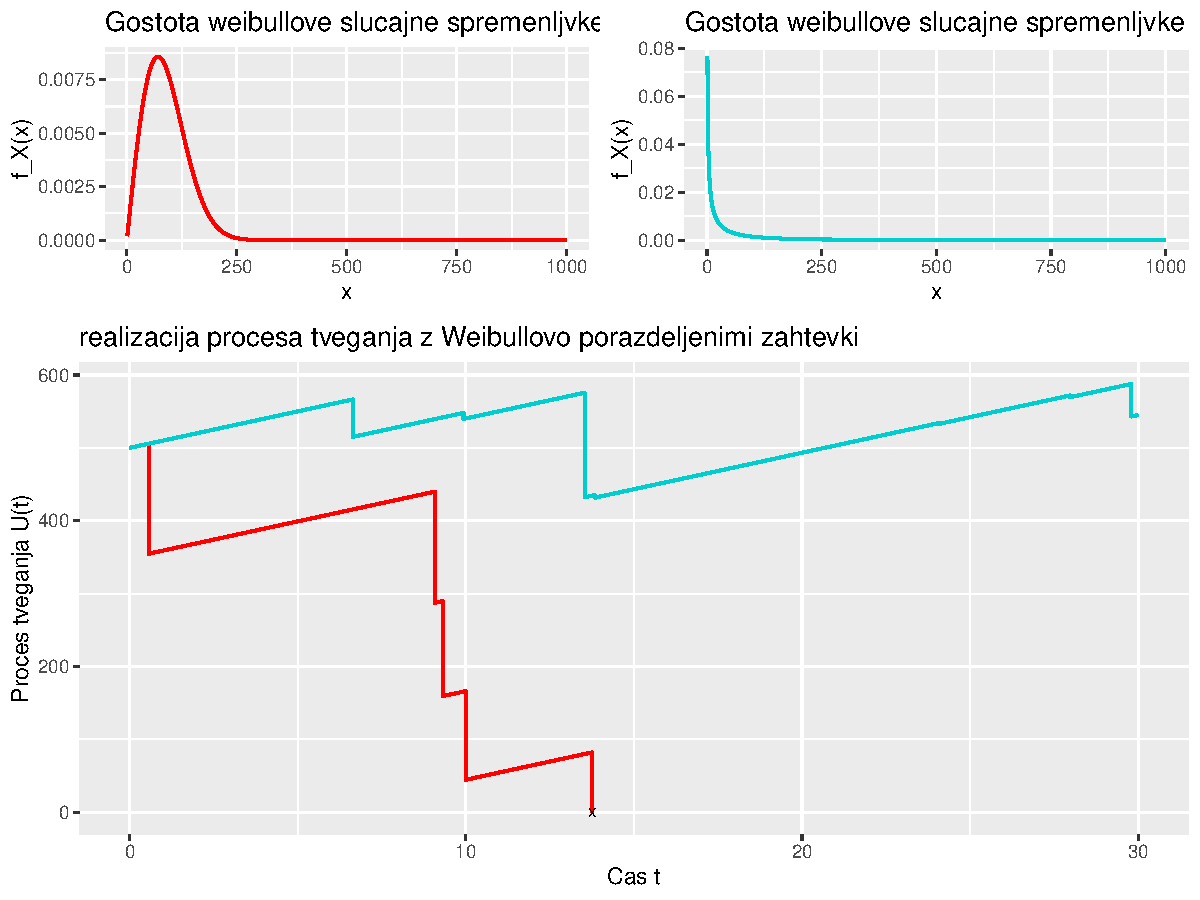
\includegraphics[width=\textwidth]{
    %            C:/Users/38651/OneDrive - Univerza v Ljubljani/Desktop/Diploma/Diplomski-seminar/GraphsAndPhotos/slika2.pdf
    %            }
    %        \caption{Histograma zahtevkov med 1.1.2015 in 1.3.2015}
    %        \label{fig:slika3}
    %    \end{figure}
%
    %    \begin{figure}[H]
    %        \centering
    %        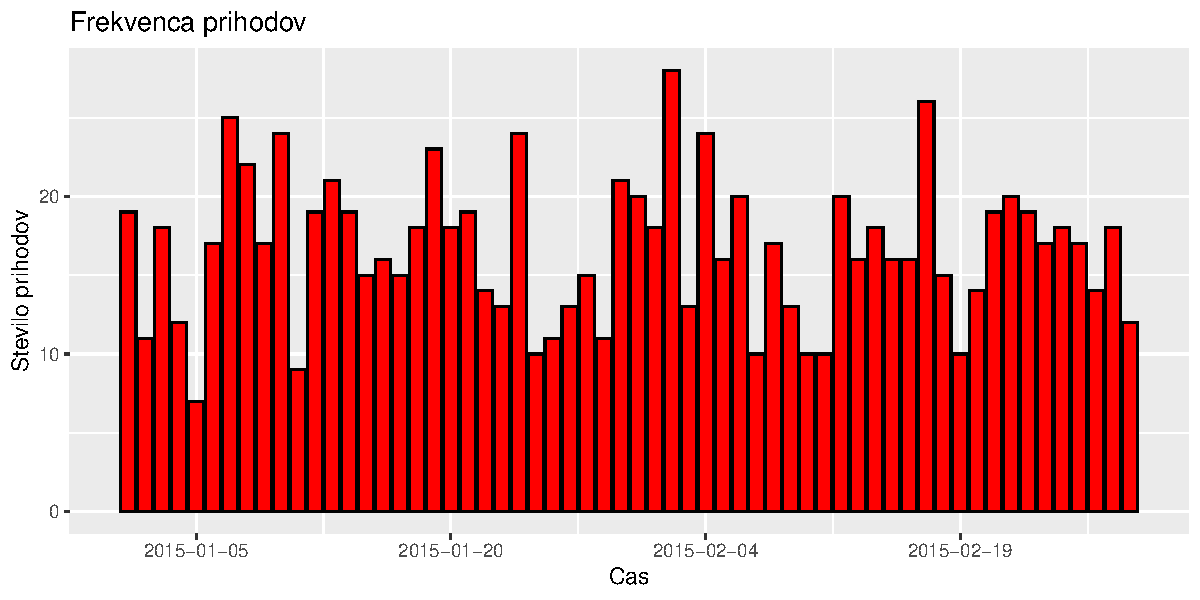
\includegraphics[width=\textwidth]{
    %            C:/Users/38651/OneDrive - Univerza v Ljubljani/Desktop/Diploma/Diplomski-seminar/GraphsAndPhotos/slika3.pdf
    %            }
    %        \caption{Stevilo prihodov zahtevkov na posamezen dan med 1.1.2015 in 1.3.2015}
    %        \label{fig:slika4}
    %    \end{figure}

        
        





\pagebreak

\section{Dostavek}
    Dostavek je namenjen predvsem za dodatne definicije in trditve, ki so bile izpu"scene v glavnem
    za namene preglednosti besdila. V primeru, "ce bralec potrebuje osve"ziti dolo"cene pojme 
    jih ve"cino lahko najde v tem razdelku.
    \begin{definicija}
        Naj bo $X$ slu"cajna spremenljivka. Potem so njena \textit{rodovna funkcija}, 
        \textit{momentno rodovna funkcija} in \textit{karakteristi"cna funkcija} definirane 
        kot 
        \begin{equation*}
            G_X(u) = \E\left[u^X\right], \quad M_X(u) = \E\left[e^{uX}\right], \quad \varphi_X(u) = \E\left[e^{iuX}\right],
        \end{equation*}
        "ce upanja obstajajo.
        \label{def:rodovneFunkcije}
    \end{definicija}

    \begin{izrek}(Lévijev izrek o kontinuiteti)
        Naj bo $(X_n)_{n\in\N}$ zaporedje slu"cajnih spremenljivk (ne nujno na istem verjetnostnem prostoru)
        in $X$ "se ena slu"cajna spremenljivka. Potem velja
        \begin{equation*}
            \varphi_{X_n}(u) \xrightarrow{n\to\infty} \varphi_X(u) \quad \text{za vsak} \ u \in \R
        \end{equation*}
        natanko tedaj, ko velja
        \begin{equation*}
            X_n \xrightarrow[n\to\infty]{d} X.
        \end{equation*}
        \label{izr:LevijevIzrek}
    \end{izrek}
    \begin{proof}
        Dokaz izreka je precej tehni"cen in ga bomo izpustili. Podroben dokaz lahko bralec najde v 
        [Fristedt, B.E., Gray L.F. (1996) A modern approach to probability theory].
    \end{proof}

    \begin{izrek}(O enoli"cnosti)
        One to one correspondence betwwen characteristic functions and distributions.
    \end{izrek}

    \begin{definicija}
        Naj bo $X$ slu"cajna spremenljivka in $F_X$ njena porazdelitev. Potem za $u\in\R$
         \textit{Laplace-Stiltjesovo transformacijo} porazdelitve $F_X$ definiramo kot
        \begin{equation*}
            \hat{F}_X(u) = \int_{-\infty}^{\infty}e^{-ux}dF_X(x).
        \end{equation*}
        \label{def:LaplaceStiltjesovaTransformacija}
    \end{definicija}

    \begin{izrek}(Tonelli (Prirejen))
        Naj bosta $X$ in $Y$ slu"cajni spremenljivki definirani vsaka na svojem verjentnostnem prostoru
        in naj imata vsaka svojo gostoto $f_X$ in $f_Y$ glede na Lebesgueovo mero.
        Potem velja
        \begin{equation*}
            \int_{\R^2}f_{X, Y}(x, y)\mathcal{L}^2(dx, dy) 
            = \int_{\R}\left(\int_{\R}f_{X, Y}(x, y)dx\right)dy = \int_{\R}\left(\int_{\R}f_{X, Y}(x, y)dy\right)dx,
        \end{equation*}
        \label{izr:TonellijevIzrek}
    \end{izrek}

    \begin{izrek}(Krepki zakon velikih "stevi)
        Naj bo $(X_n)_{n\in\N}$ zaporedje neodvisnih enako porazdeljenih
        slu"cajnih spremenljivk s pri"cakovano vrendostjo $\E\left[X_i\right] = \mu <\infty$. Potem velja
        \begin{equation*}
            \frac{X_1 + X_2 + \cdots X_n}{n}\xrightarrow[n\to\infty]{s.g.} \mu.
        \end{equation*}
        \label{izr:KrepkiZakonVelikihStevil}
    \end{izrek}

    \begin{definicija}
        Slu"cajna spremenljivka $X$ ima \textit{Weibullovo porazdelitev} s parametri $a, b > 0$, 
        "ce ima njena porazdelitev obliko 
        \begin{equation*}
            F_X(x) = 1 - e^{-\left(\tfrac{x}{b}\right)^a} \quad \text{za} \ x\geq 0
        \end{equation*}
        in gostota obliko
        \begin{equation*}
            f_X(x) = \left(\frac{a}{b}\right)\left(\frac{x}{b}\right)^{a-1}e^{-\left(\tfrac{x}{b}\right)^a} \quad \text{za} \ x\geq 0.
        \end{equation*}
        \label{def:WeibullovaPorazdelitev}
    \end{definicija}

    \begin{definicija}
        Naj bo $F$ porazdelitvena funkcija. Potem je 
        \begin{align*}
            F^{-}(x) = \int
        \end{align*}
        \textit{porazdelitev integrarnega repa F}.
        \label{def:porazdelitevZintegriranegaRepa}
    \end{definicija}

    \begin{izrek}
        izrek o sliki mere
    \end{izrek}

    \begin{trditev}
        pricakovana vrednost kot $\int_{(0, \infty)}P(X > x)dx$ za pozitivne slucajne spremenljivke
    \end{trditev}

    \begin{proof}
        dokaz trditve
    \end{proof}

    \begin{definicija}
        \textit{Prenovitveni proces} na verjentostnem protoru $(\Omega, \mathcal{F}, \Prob)$ je slu"cajni 
        proces
        karatkteriziran z zaporedjem medprihodnih "casov $(W_n)_{n\in\N}$, ki zavzamejo vrednosti
        v $\R^+\cup\{\infty\}$ in je podan z zvezo 
        \begin{equation*}
            N_t = \sum_{n=1}^{\infty}\mathbbm{1}_{\{T_n\leq t\}},
        \end{equation*}
        kjer je $T_n = W_1 + W_2 + \cdots + W_n$ "cas $n$-tega prihoda.
        \label{def:PrenovitveniProces}
    \end{definicija}

    \begin{trditev}(Neenakost Markova)
        \label{trd:neenakostMarkova}
        Za vsak $x>0$ in $u\in(-\varepsilon, \varepsilon)$ velja
        \begin{equation*}
            \Prob\left(X > x\right) \leq \frac{\E\left[X\right]}{x}.
        \end{equation*}
    \end{trditev}

    \begin{izrek}(Smith)
        neki
        \label{izr:Smith}
        
    \end{izrek}

%-----------------------------------------KONEC VSEBINE--------------------------------------------%

\section*{Slovar strokovnih izrazov}

\geslo{trajektorija}{sample path}
%
%\geslo{}{}
%


% Literatura
\begin{thebibliography}{99}
\bibitem{1}S.E. Shreve, Stochastic Calculus for Finance II: Continuous-Time Models, Springer, (2004).
\bibitem{2}S.M. Ross, Stochatic Processes: Second Edition, Wiley, (1996).
\bibitem{3}P. Embrechts, C. Klüppelberg, T. Mikosch, Modelling Extremal Events: For Insurance and Finance, Springer, (1997).
\bibitem{4}T.Mikosch, Non-Life Insurance Mathematics: An Introduction with the Poisson Process, Springer, Second Edition, (2009).
\end{thebibliography}

\end{document}